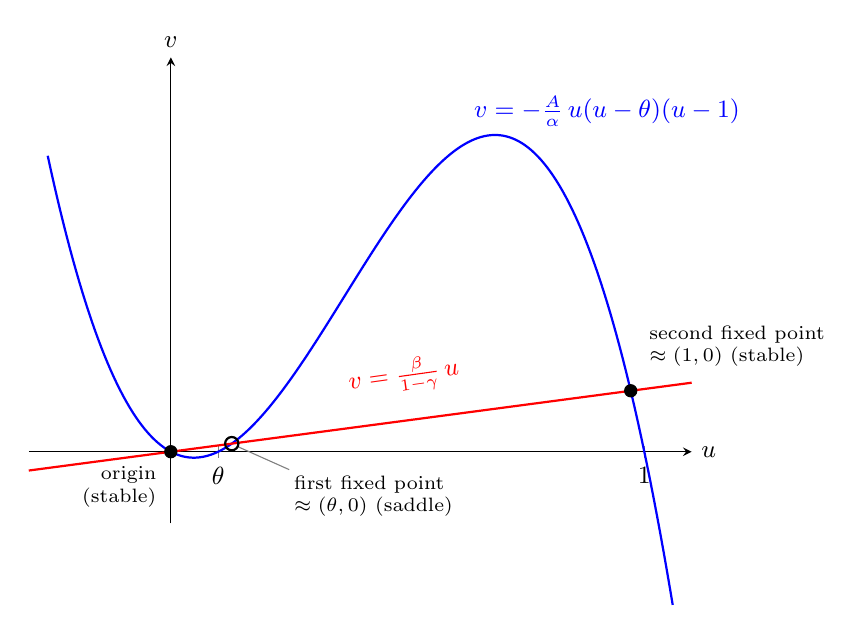
\begin{tikzpicture}
\begin{axis}[width=10cm, height=7.5cm, xmin=-0.3, xmax=1.1, ymin=-0.4, ymax=2.2,
  axis lines=middle, xlabel={$u$}, ylabel={$v$}, xtick={0.1,1}, xticklabels={$\theta$,$1$},
  ytick=\empty, tick label style={font=\small}, label style={font=\small},
  xlabel style={anchor=west}, ylabel style={anchor=south}, clip=false]
\addplot[blue, thick, domain=-0.26:1.06, samples=200] {14*x*(x-0.1)*(1-x)};
\addplot[red, thick, domain=-0.3:1.1, samples=2] {0.35*x};
\addplot[only marks, mark=*, mark size=2.2pt, black] coordinates {(0,0) (0.9713,0.3400)};
\addplot[only marks, mark=o, mark size=2.4pt, black, thick] coordinates {(0.1287,0.0450)};
\node[anchor=north east, font=\scriptsize, align=right] at (axis cs:-0.01,-0.03) {origin\\(stable)};
\node[anchor=north west, font=\scriptsize, align=left] (fp) at (axis cs:0.24,-0.08) {first fixed point\\$\approx(\theta,0)$ (saddle)};
\draw[gray] (axis cs:0.25,-0.1) -- (axis cs:0.14,0.03);
\node[anchor=south west, font=\scriptsize, align=left] at (axis cs:0.99,0.42) {second fixed point\\$\approx(1,0)$ (stable)};
\node[blue, anchor=west, font=\small] at (axis cs:0.62,1.9) {$v=-\frac{A}{\alpha}\,u(u-\theta)(u-1)$};
\node[red, anchor=south, font=\small, rotate=8] at (axis cs:0.5,0.27) {$v=\frac{\beta}{1-\gamma}\,u$};
\end{axis}
\end{tikzpicture}
